% Diagram: Directed graph with 4 labeled nodes and labeled edges.
% Coordinates: (x, y)
%   A at (0, 0)      -- source
%   B at (3, 1.5)    -- upper-right
%   C at (3, -1.5)   -- lower-right
%   D at (6, 0)      -- sink
%
% Embeds P1 (explicit dims on circles), P2, P4 (directional edge labels).
\documentclass[border=4pt]{standalone}
\usepackage{tikz}
\usetikzlibrary{positioning, arrows.meta, calc}
\begin{document}
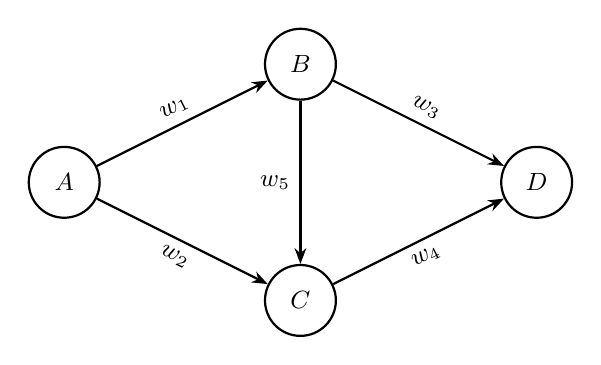
\begin{tikzpicture}[
    every node/.style={font=\small},
    vertex/.style={draw, circle, minimum size=0.9cm, inner sep=0pt, thick},
    edge/.style={-{Stealth[length=2mm]}, thick}
  ]
  \node[vertex] (A) at (0, 0)     {$A$};
  \node[vertex] (B) at (3, 1.5)   {$B$};
  \node[vertex] (C) at (3, -1.5)  {$C$};
  \node[vertex] (D) at (6, 0)     {$D$};

  \draw[edge] (A) -- (B) node[midway, above, sloped] {$w_1$};
  \draw[edge] (A) -- (C) node[midway, below, sloped] {$w_2$};
  \draw[edge] (B) -- (D) node[midway, above, sloped] {$w_3$};
  \draw[edge] (C) -- (D) node[midway, below, sloped] {$w_4$};
  \draw[edge] (B) -- (C) node[midway, left] {$w_5$};
\end{tikzpicture}
\end{document}
